\documentclass[aps,prb,twocolumn,superscriptaddress,floatfix,longbibliography,10pt]{revtex4-2}

\usepackage[utf8]{inputenc}
\usepackage[spanish]{babel}
\usepackage{graphicx}
\usepackage{amsmath}
\usepackage{subcaption}
\usepackage{wrapfig} 
\usepackage[export]{adjustbox}

\usepackage{amsmath,amssymb} % math symbols
\usepackage{bm} % bold math font
\usepackage{graphicx} % for figures
\usepackage{comment} % allows block comments
\usepackage{textcomp} % This package is just to give the text quote '
%\usepackage{ulem} % allows strikeout text, e.g. \sout{text}

\usepackage[spanish]{babel}
% By dafault, spanish changes to a comma as decimal separator; to change to a dot, you can use \decimalpoint:
\decimalpoint

\usepackage{enumitem}
\setlist{noitemsep,leftmargin=*,topsep=0pt,parsep=0pt}

\usepackage{xcolor} % \textcolor{red}{text} will be red for notes
\definecolor{lightgray}{gray}{0.6}
\definecolor{medgray}{gray}{0.4}

%Para las tablas
\usepackage{multirow}

\usepackage{hyperref}
\hypersetup{
colorlinks=true,
urlcolor= blue,
citecolor=blue,
linkcolor= blue,
bookmarks=true,
bookmarksopen=false,
}

% Code to add paragraph numbers and titles
\newif\ifptitle
\newif\ifpnumber
\newcounter{para}
\newcommand\ptitle[1]{\par\refstepcounter{para}
{\ifpnumber{\noindent\textcolor{lightgray}{\textbf{\thepara}}\indent}\fi}
{\ifptitle{\textbf{[{#1}]}}\fi}}
\ptitletrue  % comment this line to hide paragraph titles
\pnumbertrue  % comment this line to hide paragraph numbers

% minimum font size for figures
\newcommand{\minfont}{6}

% Uncomment this line if you prefer your vectors to appear as bold letters.
% By default they will appear with arrows over them.
% \renewcommand{\vec}[1]{\bm{#1}}

%Cambiar Cuadros por Tablas y lista de...
%\renewcommand{\listtablename}{Índice de tablas}
\renewcommand{\tablename}{Tabla}
\renewcommand{\date}{Fecha}

%Para importar imágenes desde una carpeta:
\graphicspath{ {C:/Users/lupam/OneDrive/Escritorio/GitHub/Metodos_Num_Fluidos_I/Guias/Informe_final/Informe/Figures} {C:/Users/lupam/OneDrive/Escritorio/GitHub/Metodos_Num_Fluidos_I/Guias/Informe_final/Programa/graficos}}

\usepackage[bottom]{footmisc} %para que las notas al pie aparezcan en la misma página

\begin{comment}

%Comandos de interés:

* Para ordenar el documento:
\section{Introducción}
\section{\label{sec:Formatting}Formatting} %label para luego hacer referencia a esa sección

\ptitle{Start writing while you experiment} %pone nombre y título al documento dependiendo de si en el header están los comandos \ptitletrue y \pnumbertrue

* Ecuaciones:
\begin{equation}
a^2+b^2=c^2 \,.
\label{eqn:Pythagoras}
\end{equation}

* Conjunto de ecuaciones:
\begin{eqnarray}
\label{eqn:diagonal}
\nonumber d & = & \sqrt{a^2 + b^2 + c^2} \\
& = & \sqrt{3^2+4^2+12^2} = 13
\end{eqnarray}

* Para hacer items / enumerar:
\begin{enumerate}
  \item
\end{enumerate}

\begin{itemize}
  \item
\end{itemize}

* Figuras:
\begin{figure}[h]
    \includegraphics[clip=true,width=\columnwidth]{pixel-compare}
    \caption{}
     \label{fig:pixels}
\end{figure}

* Conjunto de figuras:
\begin{figure}
     \centering
     \begin{subfigure}[b]{0.3\textwidth}
         \centering
         \includegraphics[width=\textwidth]{graph1}
         \caption{$y=x$}
         \label{fig:y equals x}
     \end{subfigure}
     \hfill
     \begin{subfigure}[b]{0.3\textwidth}
         \centering
         \includegraphics[width=\textwidth]{graph2}
         \caption{$y=3sinx$}
         \label{fig:three sin x}
     \end{subfigure}
     \hfill
     \begin{subfigure}[b]{0.3\textwidth}
         \centering
         \includegraphics[width=\textwidth]{graph3}
         \caption{$y=5/x$}
         \label{fig:five over x}
     \end{subfigure}
        \caption{Three simple graphs}
        \label{fig:three graphs}
\end{figure}


* Para hacer referencias a fórmulas, tablas, secciones, ... dentro del documento:
\ref{tab:spacing}

* Para citar
Elementos de .bib
\cite{WhitesidesAdvMat2004}
url
\url{http://www.mendeley.com/}\\

* Agradecimientos:
\begin{acknowledgments}
We acknowledge advice from Jessie Zhang and Harry Pirie to produce Fig.\ \ref{fig:pixels}.
\end{acknowledgments}

* Apéndice:
\appendix
\section{\label{app:Mendeley}Mendeley}

* Bibliografía:
\bibliography{Hoffman-example-paper}

\end{comment}



\begin{document}

% Allows to rewrite the same title in the supplement
\newcommand{\mytitle}{\textcolor{red}{Título??}}

\title{\mytitle}

\author{Pablo Chehade \\
    \small \textit{pablo.chehade@ib.edu.ar} \\
    \small \textit{Métodos Numéricos en Fluidos I, Instituto Balseiro, CNEA-UNCuyo, Bariloche, Argentina, 2022} \\}


\begin{abstract}

\begin{itemize}
  \item Se estudiaron métodos numéricos espaciales y de evolución temporal para resolver el problema de la cavidad cuadrada hidrodinámica bidimensional.
  \item Se tiene en cuenta la ecuación de momentos y la de conservación de masa. Este tiene un término advectivo, uno difusivo.
  \item Se resolvió mediante el método de volumenes finitos y algoritmo simpler calculando presión y velocidades diferidas? con grilla desplazada.
  \item En primer lugar, se estudió la dependencia de la solución en el estado estacionario con respecto al paso temporal.
  \item Se planteó un algoritmo para minimizar el costo computacional para encontrar el estado estacionario con un error menor al 5 \%
  \item Se evaluó el efecto de los pasos internos del algoritmo simpler
  \item En segundo lugar, se estudió el impacto en el estacionario del esquema espacial en el término advectivo empleando distintos números de Reynolds. En particular, se utilizaron diferencias centradas de orden 2, Up-wind de orden uno y el esquema QUICK de orden \textcolor{red}{?}
  \item Además, se estudió el orden de convergencia espacial de Up-wind de primer orden en referencia al mejor esquema advectivo
  \item Se estudió el efecto del método de evolución temporal, evaluando el estado transitorio de la solución mediante los métodos Euler Implícito y Crank-Nicholson
\end{itemize}


\end{abstract}

\maketitle

\section{Introducción}

\ptitle{¿Por qué es importante resolver problemas de fluidos numéricamente? Rtas en la primera clase}

\begin{itemize}
  \item Una gran parte de los problemas de mecánica de fluidos no son resolubles analíticamente
  \item En algunos de los problemas es posible realizar experimentos. Sin embargo, estos traen aparejados un gran costo operativo y dificultades para realizar las mediciones \textcolor{red}{ref clase 1}
  \item Una alternativa más rápida y de menor costo es resolver estos problemas numéricamente, con las dificultades que esto conlleva. Tal es el caso de los errores de aproximación numérica y el costo computacional, que puede ser aún así más barato que hacer el experimento
  \item Aun así, en los últimos años la resolución numérica de ecuaciones es aceptada y está ganando preponderancia
\end{itemize}

\ptitle{Explicar el problema de la cavidad cuadrada hidrodinámica bidimensional}
\begin{itemize}
  \item Un problema muy estudiado desde el punto de vista numérico en mecánica de fluidos es el de la cavidad cuadrada hidrodinámica bidimensional, también conocida como Shear-drien cavity flow
  \item Consiste en una cavidad cuadrada bidimensional de lado $L$ que contiene un fluido incompresible de viscocidad $\nu$. Las condiciones de borde son de no deslizamiento en todas las paredes excepto en la horizontal superior. Sea $\vec{V}(x,y) = (u(x,y), v(x,y))$ la velocidad en el punto $(x,y)$, las condiciones anteriores se traducen en $\vec{V}(x,0) = \vec{V}(0,y) = \vec{V}(L,y) = (0,0)$ y $\vec{V}(x,L) = (U_0,0)$
  \item En la figura \ref{fig:esquema_cavidad_cuadrada} se muestra un esquema del problema
\end{itemize}

\begin{figure}[h]
  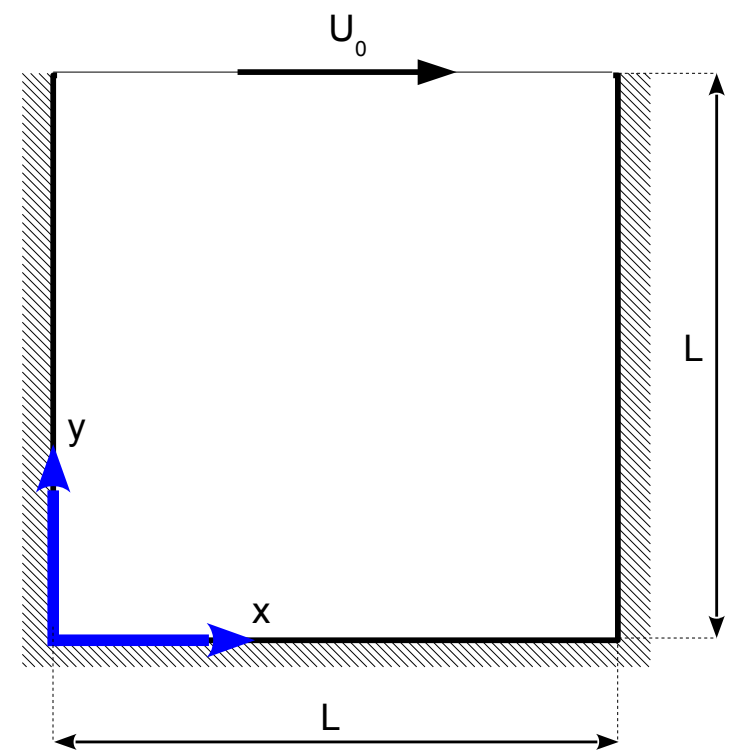
\includegraphics[clip=true,width=\columnwidth]{esquema_cavidad_cuadrada.png}
  \caption{}
   \label{fig:esquema_cavidad_cuadrada}
\end{figure}


\ptitle{Explicación de las ecuaciones involucradas}
\begin{itemize}
  \item Las variables de interés son la presión y la velocidad vertical y horizontal
  \item Se cuentan con tres ecuaciones diferenciales:
  \item En primer lugar, las dos ecuaciones de conservación de momento en direcciones vertical y horizontal que, adimensionales, son
  \[\frac{\partial u}{\partial t} + \frac{\partial (u u)}{\partial x} + \frac{\partial (u v)}{\partial y} = - \frac{\partial p}{\partial x} + \frac{1}{Re} \left ( \frac{\partial^2 u}{\partial x^2} + \frac{\partial^2 u}{\partial y^2} \right ) \]
  \[\frac{\partial v}{\partial t} + \frac{\partial (u v)}{\partial x} + \frac{\partial (v v)}{\partial y} = - \frac{\partial p}{\partial y} + \frac{1}{Re} \left ( \frac{\partial^2 v}{\partial x^2} + \frac{\partial^2 v}{\partial y^2} \right ) \]
  donde $Re = U_0L/\nu$

  \item Nombrar cada término (temporal, advectivo, de presión y difusivo)
  \item En segundo lugar, la ecuación de conservación de masa que para fluido incompresible es
  \[\bigtriangledown \bullet \vec{V} = \frac{\partial u}{\partial x} + \frac{\partial v}{\partial y} = 0  \]

  \item en base a esa ecuación se dice que el campo de velocidades tiene "divergencia libre"
  \item Las soluciones dependen de Re
\end{itemize}

\section{Métodos Numéricos}

\ptitle{Resumen}
\begin{itemize}
  \item Para resolver el sistema de ecuaciones diferenciales es necesario discretizar el dominio y plantear esquemas numéricos para las ecuaciones. En cuanto al primero, es necesario diferenciar entre dominio espacial y temporal.
  \item En cuanto al segundo, se emplearon volúmenes finitos con el objetivo de asegurar la conservación de masa \textcolor{red}{?} y distintos métodos espaciales y temporales para cada término.
\end{itemize}

\ptitle{Discretización espacial}
\begin{itemize}
  \item El dominio espacial se discretiza ... 
  \item Copiar lo que está en el pdf de la cátedra
  \item \cite{Notas_materia}
\end{itemize}

\ptitle{Grilla desplazada}
\begin{itemize}
  \item Copiar lo que está en el pdf de la cátedra
\end{itemize}
\begin{figure}
  \centering
  \begin{subfigure}[b]{0.25\textwidth}
      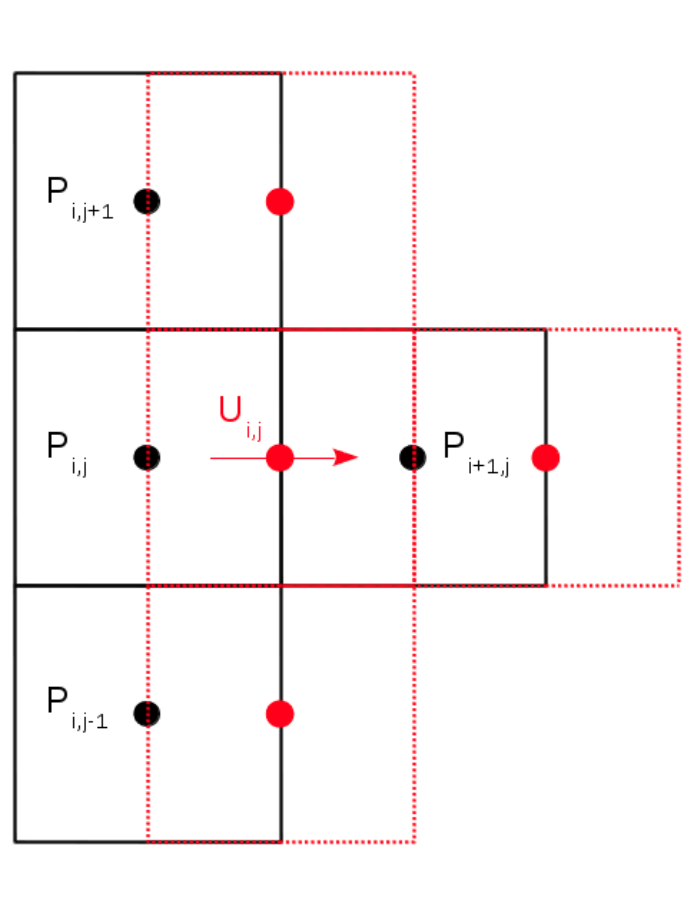
\includegraphics[width=\textwidth]{grilla_diferida_u.png}
      \caption{}
      \label{fig:grilla_diferida_u}
  \end{subfigure}
  \hfill
  \begin{subfigure}[b]{0.2\textwidth}
      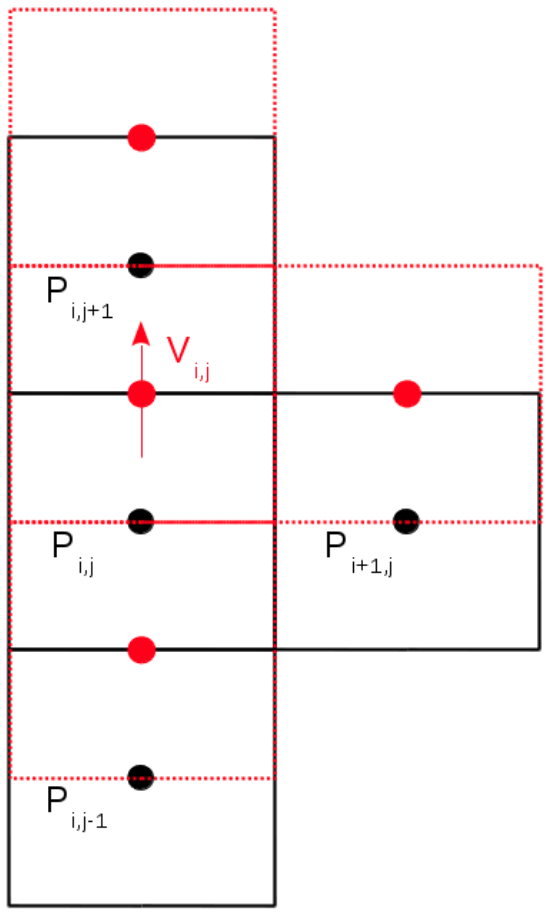
\includegraphics[width=\textwidth]{grilla_diferida_v}
      \caption{}
      \label{fig:grilla_diferida_v}
  \end{subfigure}
     \caption{Grillas diferidas. Figuras extraídas de \cite{Notas_materia}}
     \label{fig:grillas_diferidas}
\end{figure}


\ptitle{Discretización temporal}
\begin{itemize}
  \item En cuando al dominio temporal, la variable temporal se discretizó en puntos equiespaciados $t_n = n \Delta t$ con $n = 0,1,\dots,N$ con $\Delta t = t_{max}/N$
\end{itemize}


\ptitle{Costo computacional y elección de dt}
\begin{itemize}
  \item Debido a la cantidad de variables involucradas y dependiendo del número de pasos de tiempo a realizar, el costo computacional puede ser alto.
  \item Un modo de minimizarlo es eligiendo n1 lo suficientemente pequeño para que el error sea menor a una tolerancia determinada, aunque para esto es necesario conocer al menos la solución exacta, lo cual no siempre se tiene
  \item Otra alternativa es elegir $N$ en base a un criterio de convergencia: si la solución tiende a un estacionario independiente del tiempo, entonces avanzamos la solución hasta que, por ejemplo, CONDICIÓN SOBRE DERIVADAS
  \item Si solo es de interés la solución en el estado estacionario, otro modo de atacar el problema es eligiendo dt para que el problema converja rápido a pesar de tener un estado transitorio lejos de la solución exacta. Esto último se basa en la hipótesis de que la solución no depende del paso de tiempo
  \item En este trabajo se estudiaron ambos métodos, eligiendo n1 de modo que el error sea menor a una tolerancia de 1e-5 y proponiendo un algoritmo para elegir dt de modo de minimizar el costo computacional.
  \item No describir el algoritmo
\end{itemize}




\ptitle{Algoritmo simpler simplificadamente}
\begin{itemize}
  \item \cite{Patankar}
  \item Es un algoritmo segregado o de paso fraccionado. Esto último en el sentido de que se calculan por separado $\vec{v}$ y $p$.
  \item Permite calcular la velocidad con divergencia libre (cumple la conservación de masa) y la presión en cada paso de tiempo a partir de un guess, el cual suele ser la solución del paso anterior. \textcolor{red}{es así, no?}
  \item Se propone que determinados términos de la ecuación se pueden estimar con el paso anterior. Se calcula la presión de modo de que el nuevo campo de velocidades tenga divergencia libre. Luego se calcula el campo de velocidades empleando esta nueva presión, obteniendo un campo que no necesariamente tiene divergencia libre. Posteriormente, se vuelve a calcular la presión de modo que el nuevo campo de velocidades tenga divergencia libre, empleando como guess el campo de velocidades calculado. Este proceso es un paso del algoritmo simpler.
  \item En el link \url{https://www.cfd-online.com/Wiki/SIMPLER_algorithm_-_SIMPLE_-_Revised} se explica el procedimiento bien resumido y sin ecuaciones.
  \item La exactitud de la solución depende del número de pasos internos realizados en el algoritmo, que pueden ser tantos como uno quiera aunque aumenta el costo computacional
\end{itemize}



\textcolor{red}{Es necesario explicar cómo discretizar las ecuaciones de momento? Sería copiar textual el desarrollo hecho en la penúltima clase. Le pregunté a Federico}
\textcolor{red}{Plantear lo siguiente luego de que Federico me halla respondido}

\ptitle{Esquemas numéricos posibles para cada término}
\begin{itemize}
  \item Para cada término de las ecuaciones de momento, se pueden plantear distintos esquemas numéricos. En este trabajo se estudiaron los siguientes:
  \begin{itemize}
    \item Para la parte temporal, se emplearon los esquemas de Euler implícito y de Crank-Nicolson.
  \end{itemize}
\end{itemize}

\ptitle{Término advectivo. Explicar cada método numérico}
\begin{itemize}
  \item 
\end{itemize}

\ptitle{Término temporal. Explicar cada método numérico}
\begin{itemize}
  \item 
\end{itemize}



\ptitle{Resumen de lo que se va a estudiar}
\begin{itemize}
  \item En primer lugar, se estudió la dependencia de la solución en el estado estacionario con respecto al paso temporal.
  \item Se planteó un algoritmo para minimizar el costo computacional para encontrar el estado estacionario con un error menor al 5 \%
  \item Se evaluó el efecto de los pasos internos del algoritmo simpler
  \item En segundo lugar, se estudió el impacto en el estacionario del esquema espacial en el término advectivo empleando distintos números de Reynolds. En particular, se utilizaron diferencias centradas de orden 2, Up-wind de orden uno y el esquema QUICK de orden \textcolor{red}{?}
  \item Además, se estudió el orden de convergencia espacial de Up-wind de primer orden en referencia al mejor esquema advectivo
  \item Se estudió el efecto del método de evolución temporal, evaluando el estado transitorio de la solución mediante los métodos Euler Implícito y Crank-Nicholson
\end{itemize}





\begin{itemize}
  \item \textcolor{red}{En todos los casos se usó una tolerancia para el estado estacionario de 1e-5}
\end{itemize}

\section{Resultados y discusión}


\subsection{Dependencia del estado estacionario con el paso dt}

En primer lugar, se analizó la dependencia del estado estacionario en relación al paso de evolución temporal. Se calculó $u(0.5,0.5)$ y $v(0.5,0.5)$ para $Re = 1000$, $n_1 = 20$ y distintos $\Delta t$ entre $0.005$ y $20$. Como método numérico para el término advectivo se empleó diferencias centradas de orden 2 y como método temporal, Euler implícito. En la figura \ref{fig:a_vel_vs_dt} se grafican los resultados obtenidos respecto al valor correspondiente al menor $\Delta t$ en valor absoluto. Se observa una diferencia entre los valores obtenidos del orden 

\begin{figure}[h]
  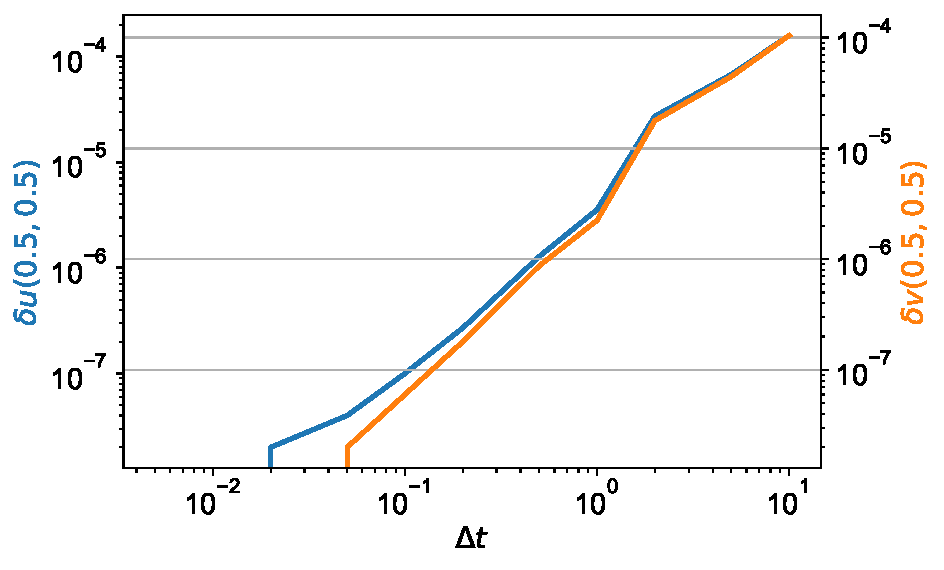
\includegraphics[clip=true,width=\columnwidth]{a_vel_vs_dt.pdf}
  \caption{}
   \label{fig:a_vel_vs_dt}
\end{figure}

Se calculó para cada caso la desviación estándar de la velocidad normalizada por el valor promedio

\subsection{Elección de dt}
Describir el algoritmo

\subsection{dt para distintos lsimpler}

Estaría bueno dar para cada caso el máximo dt posible y el que me da mi algoritmo

\subsection{Término advectivo}

Se implementó para el término advectivo los esquemas DC2, UP1 y QUICK. Se resolvió el problema para $Re = 100, 1000 \, \mathrm{y} \, 5000$ y para $n1 = 20, 40 \, \mathrm{y} \, 80$. Se calculó para cada caso el error relativo respecto a los resultados de Guia.
$tol_estacionario = 1e-5$

\begin{figure}
  \centering
  \begin{subfigure}[b]{0.3\textwidth}
      \centering
      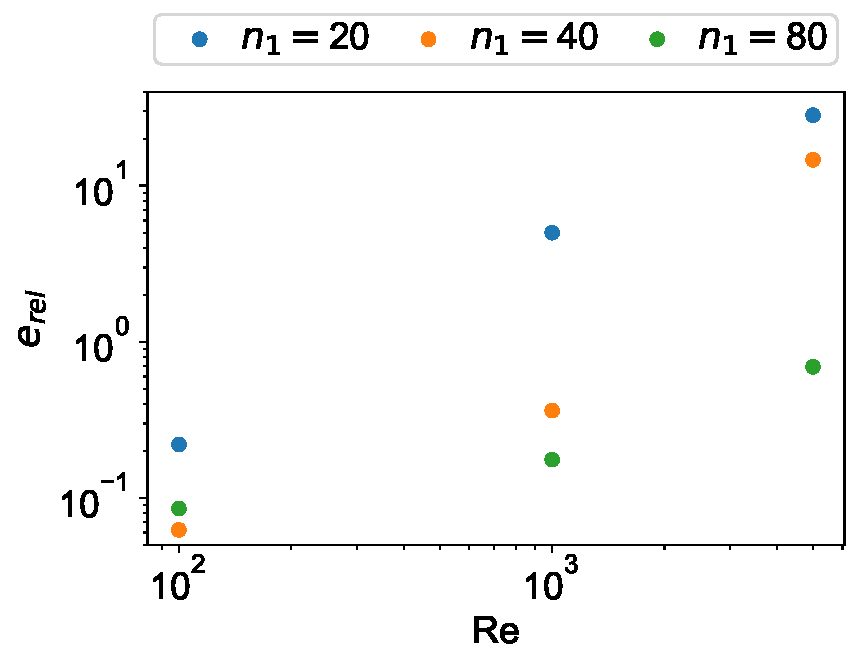
\includegraphics[width=\textwidth]{termino_adv_DC2.pdf}
      \caption{}
      \label{fig:termino_adv_DC2}
  \end{subfigure}
  \hfill
  \begin{subfigure}[b]{0.3\textwidth}
      \centering
      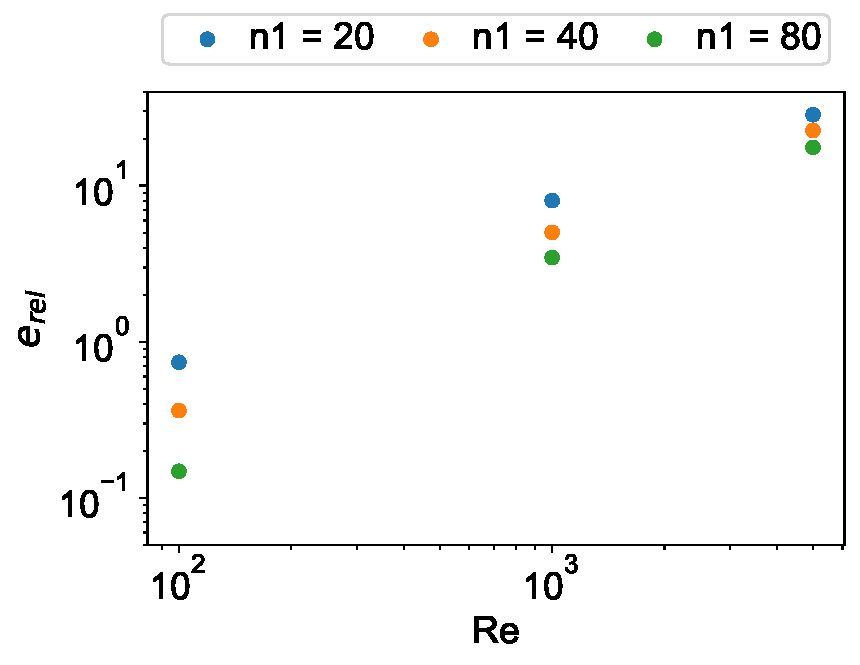
\includegraphics[width=\textwidth]{termino_adv_UP1.pdf}
      \caption{}
      \label{fig:termino_adv_UP1}
  \end{subfigure}
  \hfill
  \begin{subfigure}[b]{0.3\textwidth}
      \centering
      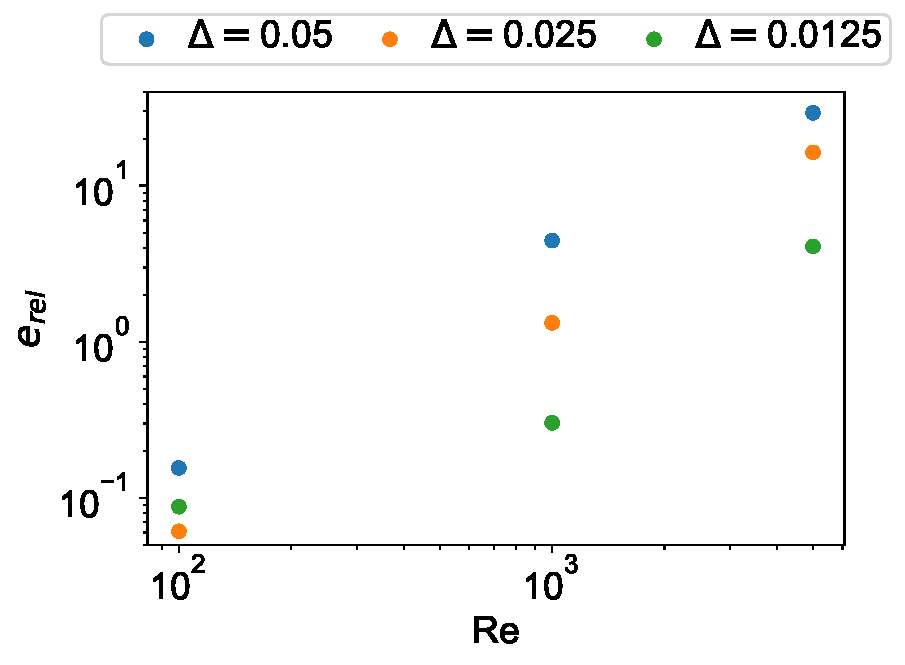
\includegraphics[width=\textwidth]{termino_adv_QUICK.pdf}
      \caption{}
      \label{fig:termino_adv_QUICK}
  \end{subfigure}
     \caption{Termino advectivo}
     \label{fig:termino_advectivo}
\end{figure}

\textcolor{blue}{Tabla con resultados}

\textcolor{red}{Duda: es necesario reportar el dt en cada caso?}

\subsection{Orden de convergencia espacial de UP1}

Se calculó $u(0.5)$ y $v(0.5)$ para $Re = 1$ y $Re = 1000$ con $n1 = 80$ y esquema QUICK. Se consideró este valor como la solución exacta. Luego, se calcularon las mismas velocidades para distintos n1 y se calculó el error respecto a la solución numérica considerada como la exacta

\begin{figure}[h]
  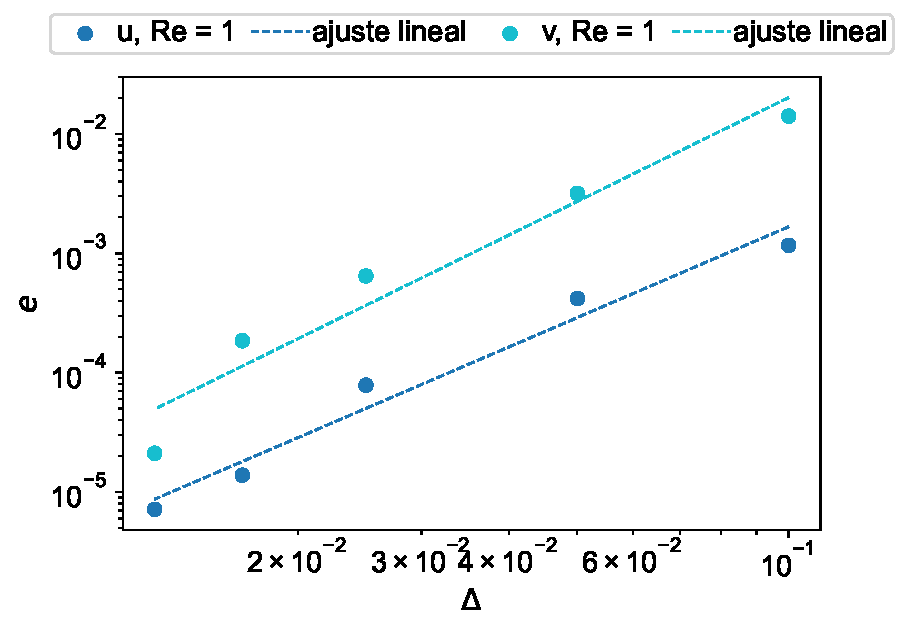
\includegraphics[clip=true,width=\columnwidth]{error_UP1_n1_vs_Re.pdf}
  \caption{}
   \label{fig:error_UP1_n1_vs_Re}
\end{figure}

\suvsection{Esquema temporal con solución dependiente del tiempo}

\textcolor{blue}{Evolución temporal con EI y CN.}





\section{Conclusión}

\bibliography{Chehade_final.bib}

\end{document}





